
Les résultats présentés dans cette thèse portent principalement sur la détermination des
contributions des sources de PO à travers un modèle linéaire.  Cependant, le contournement
des limitations soulevées et certaines pistes de travail dans le cadre plus général de la
recherche d'un meilleur indicateur de l'exposition à travers la métrique du potentiel
oxydant ont également commencés à être abordés.  Ces travaux, pleinement intégrés au
projet de recherche de l'équipe CHIANTI, s'appuient en partie sur mes résultats de thèse et
en sont sa continuité logique ou explorent des axes volontairement écartés de ma thèse.
Mon implication y est donc importante et continuera de l'être lors de mes recherches
futures.

Dans ce chapitre, deux des axes principaux qui constitueront mon travail post-thèse sont
développés et des résultats déjà obtenus sont brièvement exposés.

\section{Vers une prise en compte améliorée de l'exposition sanitaire}%

Au cours de ma thèse, plusieurs questions ont pu être posées et certaines réponses
apportées.  Cependant, le choix a été fait de se limiter principalement à l'estimation des
sources du potentiel oxydant à travers le modèle source-récepteur PMF. Bien qu'apportant
des résultats éclairants sur la dynamique des différents tests de PO, plusieurs aspects ont
été volontairement écartés de ces études.

Premièrement, l'utilisation des modèles site-récepteur limite nécessairement la couverture
spatiale et temporelle à quelques sites d'études et années de mesures. Or la
généralisation d'une estimation des mesures de PO en tous points spatio-temporels est
souhaitable lorsque l'on s'intéresse à coupler dans une même étude mesures
épidémiologiques et qualité de l'air, et elle est indispensable si l'on souhaite faire de
la prévision dans le futur.

Deuxièmement, la méthode utilisée pour estimer un PO par source d'émission de particules
présente un développement mathématique linéaire. Or, on sait que le PO ne réagit pas de
manière linéaire à la masse des composés chimiques et que la génération des ROS dans les
fluides pulmonaires n'est pas linéaire pour tous les composés atmosphériques. Si ce modèle
présente une première approximation plutôt valable pour les basses masses, il est, par
construction, limité et biaisé.  Il existe cependant des modèles d'inversion non-linéaire
qui permettraient la prise en compte des interactions entre sources et composés chimiques
dans l'estimation des sources de PO.

Finalement, jusqu'à présent seuls des prélèvements en air extérieur ont été considérés.
Or, en moyenne, un européen passe la majeur partie de son temps en espace clos intérieur
(domicile, appartement, bureau, voiture, etc.).  La représentativité des mesures en air
extérieur comme référence de l'exposition de la population n'est donc peut-être pas
suffisante.

Les résultats des premiers travaux qui ont débuté sur ces trois aspects, auxquels je
participe, sont présentés ci dessous.

\section{Spatialisation du PO}

\subsection{Estimation du PO à partir de la concentration massique des PM}

\subsubsection{Principe général}

Ayant attribué un PO intrinsèque aux sources déterminées sur un site récepteur, il est
possible de généraliser la prédiction des valeurs de PO sur ce site en estimant une
contribution moyenne mensuelle de chacune des sources. Ainsi, on peut envisager un ``gap
filling'' des mesures de PO. Par exemple, le site de GRE-fr n'a été échantilloné qu'un
jour sur trois, mais la station d'AtmoAURA enregistre les mesures journalières des
concentrations de \PMdix. Il est donc envisageable, en utilisant les contributions
relatives des sources estimées sur ce site, de ``prédire'' un \POAAv{} et \PODTTv{} pour
les jours manquants.

Il est aussi possible d'aller plus loins dans la réflexion. Dans cette thèse, deux
synthèses nationales grande échelle ont été faites : 1) estimation des contributions des
sources de PM à la masse \autocite{weberComparison2019}
(chapitre~\ref{cha:approfondissement_des_connaissances_des_sources_des_pm}) et 2) attribution du PO intrinsèque à
chacune des sources de PM majoritairement déterminées \autocite{weberSourceinprep.}
(chapitre~\ref{cha:estimation_des_sources_de_PO}).

Ainsi, en première approximation et en supposant une généralité suffisante des 2
synthèses précédentes, il est possible d'estimer la contribution relative mensuelle
moyenne des différentes sources à la masse totale des PM pour un site quelconque.  Puis,
connaissant le PO intrinsèque (i.e. par microgramme de PM) de chacune de ces sources, une
estimation au premier ordre du PO est envisageable.  La conséquence est que pour chaque
valeur de concentration de \PMdix{} il est possible d'estimer une valeur de PO associée.

Formellement, cela revient à généraliser la figure 6 de \cite{weberSourceinprep.} à un
site quelconque et donc à attribuer les \OPm{} (\si{\opm}) par microgramme de \PMdix{}
mensuels présentés dans le tableau~\ref{tab:monthly_opi}.

\begin{table}[ht]
    \centering
    \small
    \begin{tabular}{lrrrrrrrrrrrr}
    \toprule
    month   & 1     & 2     & 3     & 4     & 5     & 6     & 7     & 8     & 9     & 10    & 11    & 12 \\ \midrule
    \OPAAm  & 0.114 & 0.090 & 0.066 & 0.049 & 0.043 & 0.033 & 0.037 & 0.042 & 0.051 & 0.077 & 0.104 & 0.124 \\
    \OPDTTm & 0.115 & 0.104 & 0.099 & 0.099 & 0.105 & 0.107 & 0.109 & 0.111 & 0.113 & 0.125 & 0.119 & 0.119 \\
    \bottomrule
    \end{tabular}
    \caption{Approximation du PO intrinsèque en \si{\opm} (i.e. par microgramme) de
        \PMdix{} mensuel en ne prenant en compte que les 8 sources de PM majoritaires
        déterminées par \cite{weberSourceinprep.}
    }
    \label{tab:monthly_opi}
\end{table}

Cette méthode possède trois hypothèses et limitations fortes : 
\begin{itemize}
    \item Les contributions relatives des sources sont moyennées mensuellement d'après un
        ensemble de 15 sites de mesures, de typologie plutôt urbaine, et donc non
        nécessairement représentative de l'ensemble des situations possibles ;
    \item Le PO intrinsèque de chacune de ces sources présente en réalité une variabilité
        plus ou moins importante, et une fois de plus il est estimé à partir d'un ensemble de
        sites de typologie plutôt urbaine ;
    \item Il n'est pas pris en compte la spécificité du site en question (source atypique,
        topographie, climat...) ni la possible évolution du PO intrinsèque des sources qui
        serait liés à une évolution du profil chimique (renouvellement de parc automobile,
        etc.).
\end{itemize}

Cette méthode simple présente néanmoins l'avantage de pouvoir estimer depuis une concentration massique
des \PMdix{} une valeur au premier ordre de \POAAv{} et \PODTTv, qu'il s'agisse d'un site
de mesure ``standard'' avec TEOM-FDMS ou d'une cartographie issue de prévisions
déterministes d'un modèle CTM, ou encore de mesures satellitaires.

Aussi, au fur et à mesure de la parution future de nouvelles études, cette technique pourra être 
affinée en ne sélectionnant que des sites de même typologie ou
environnement (rural, vallée alpine, trafic, etc.) aussi bien pour la partie d'estimation
de la contribution des sources aux \PMdix{} que pour la partie attribution d'un PO
intrinsèque par source.

Enfin, il est possible de propager la variabilité aussi bien de la contribution mensuelle
moyenne de chacune des sources que de leur PO intrinsèque dans cette méthode. Ce travail n'a
pas encore été entamé, mais nous disposons de l'ensemble des informations nécessaires pour
cela.

\begin{tcolorbox}[colback=red!5!white,colframe=Melon,title=Note]
    Cette méthode est aussi rendue disponible grâce au développement du module python
    \href{https://gricad-gitlab.univ-grenoble-alpes.fr/pmall/pyopestimator}{pyOPestimator},
    disponible sur PyPi\footnote{\url{https://pypi.org/project/pyOPestimator/}} et sur la
    forge de l'université de
    grenoble\footnote{\url{https://gricad-gitlab.univ-grenoble-alpes.fr/pmall/pyopestimator}}.

    Il est également possible d'utiliser \url{http://getopstandop.u-ga.fr/estimate},
    permettant d'estimer directement en ligne le \POAAv{} et \PODTTv{} de n'importe quelle
    série de mesures de concentrations massiques de \PMdix.
\end{tcolorbox}

\subsubsection{Application sur un site urbain hors des études précédentes}

Afin de tester la faisabilité et la généralisation suffisante des synthèses nationales,
cette méthode d'estimation au premier ordre du PO a été appliquée sur le site de Zurich,
pour les échantillons de l'étude en cours avec l'EMPA. 
L'estimation a été faite en n'utilisant que les huit sources majoritaires issues de la
synthèse française, et leur \OPm{} moyen pour l'ensemble des quinze sites français.

Les \POAAv{} et \PODTTv{} mesurés sur les échantillons et estimés par cette méthode sont
présentés figure~\ref{fig:figures/chapter05/pyopestimator_EMPA_ZURICH} pour tous les
échantillons journaliers collectés.  Les cycles saisonniers sont bien retrouvés et les
amplitudes respectées. Cependant et comme attendu, certains évènements peu fréquents sont
mal estimés. Au final, des corrélations (Pearson) respectives de 0.74 et 0.80 pour le
\POAAv{} et \PODTTv{} sont obtenues.  Considérant les grandes approximations faites par cette
méthode, ce résultat présente donc des performances étonnantes.

On remarque également -- conformément à ce que les études de regression linéaires
multiples montraient déjà -- une tendance à la sous-estimation des fortes valeurs de PO,
suggérant une fois de plus la présence de phénomènes non linéaires.

\begin{figure}[ht]
    \centering
    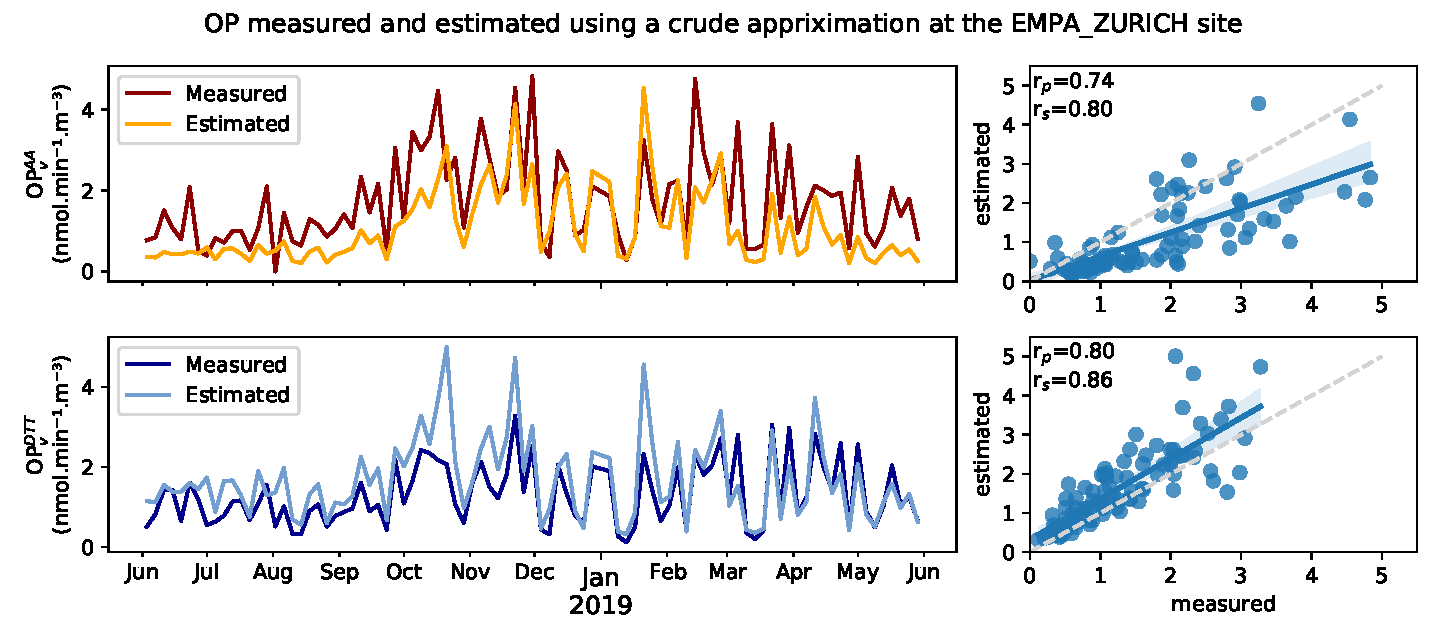
\includegraphics[width=1.0\linewidth]{figures/chapter05/pyopestimator_EMPA_ZURICH.pdf}
    \caption{\POAAv{} (haut) et \PODTTv{} (bas) mesurés et estimés sur le site de l'EMPA
    de Zurich. $r_p$ et $r_s$ sont respectivement les coefficients corrélations de Pearson
et Spearman.}
    \label{fig:figures/chapter05/pyopestimator_EMPA_ZURICH}
\end{figure}

% \begin{figure}[ht]
%     \centering
%     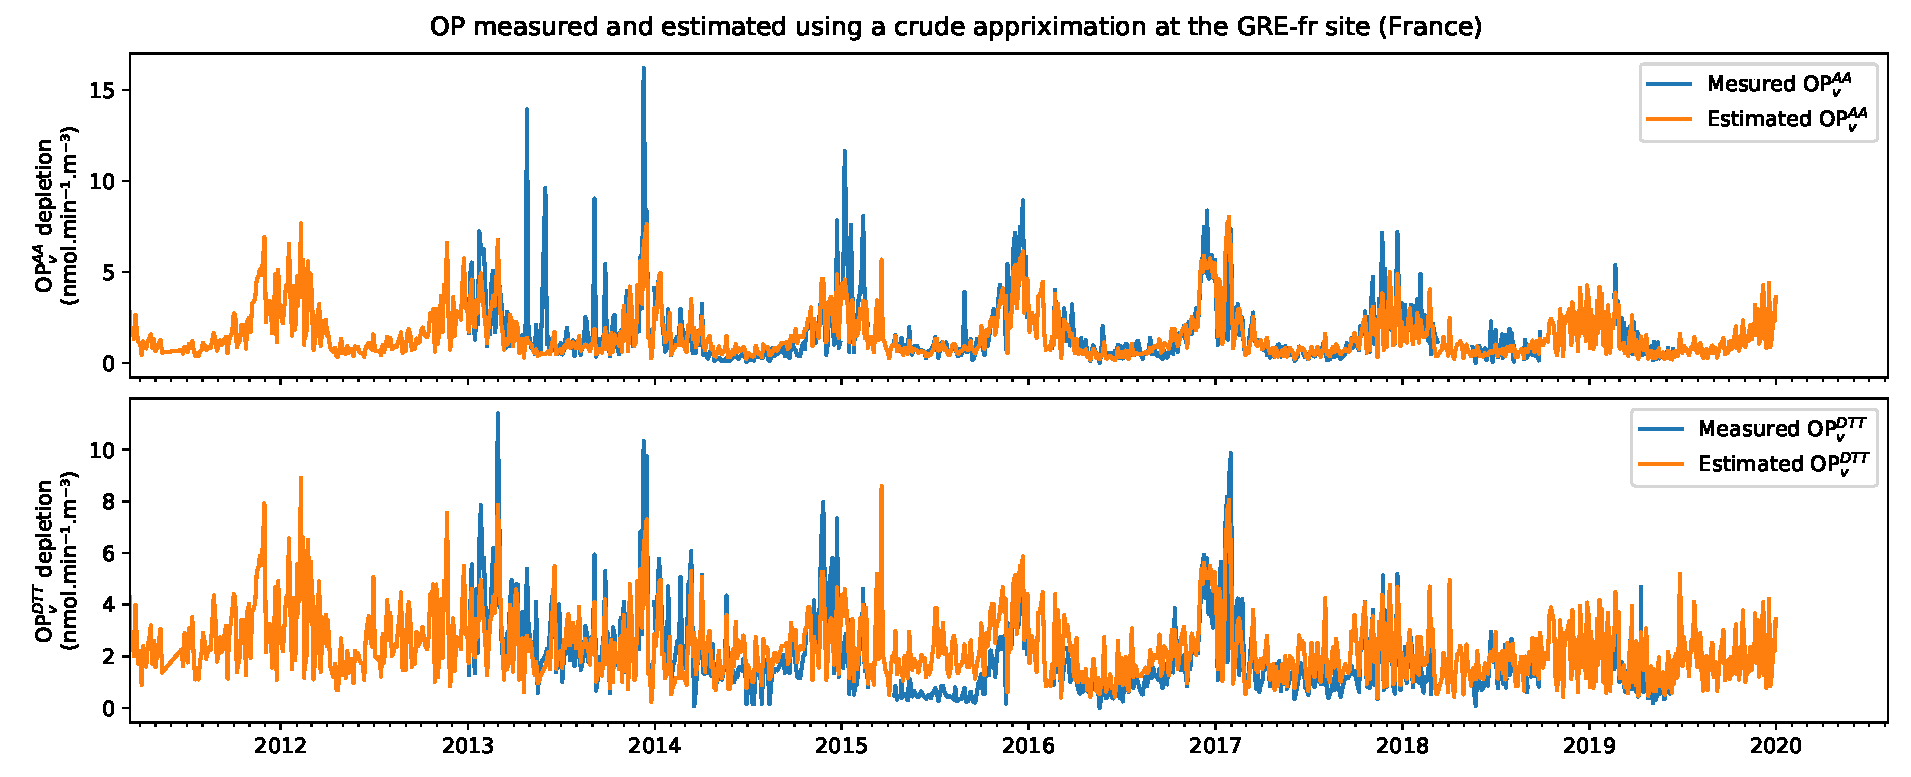
\includegraphics[width=1.0\textwidth]{figures/chapter05/OPGRE-fr_estimated.pdf}
%     \caption{\POAAv{} (haut) et \PODTTv{} (bas) estimés en orange et mesurés en bleu sur le site de GRE-fr depuis 2011.}
%     \label{fig:OPGRE-fr-estimated}
% \end{figure}
%  

\subsubsection{Applicatibilité du ``gap-filling'' sur GRE-fr}

La même analyse est conduite sur le site de GRE-fr, afin d'estimer la faisabilité du
``gap-filling'', en prenant en compte l'intégralité des mesures annuelles de masse des
\PMdix{} disponibles de la station d'AtmoAURA (entre 2013 et début 2020). La prise en compte de toutes ces mesures
nous affranchit du biais de sélection présent du fait de la fréquence d'échantillonage et
d'analyse sur filtre lors de l'estimation de la contribution annuelle des sources au
potentiel oxydant.

\paragraph{Confrontation aux mesures}%
\label{par:confrontation_aux_mesures}

La confrontation entre estimations des PO et leurs mesures (déja réalisées sur un grand
nombre d'échantillons de cette série cf. figure~\ref{fig:TSGREfr} du
chapitre~\ref{cha:estimation_des_sources_de_PO}) sur l'ensemble de cette série de mesure
(entre 2013 et début 2020) est présentée figure~\ref{fig:OPGRE-fr-estimated_scatter}. Elle
montre que ces résultats sont là encore satisfaisants (coefficient de pearson respectivement de r=0.75 et r=0.79
pour le \POAAv{} et \PODTTv).

\begin{figure}[ht]
    \centering
    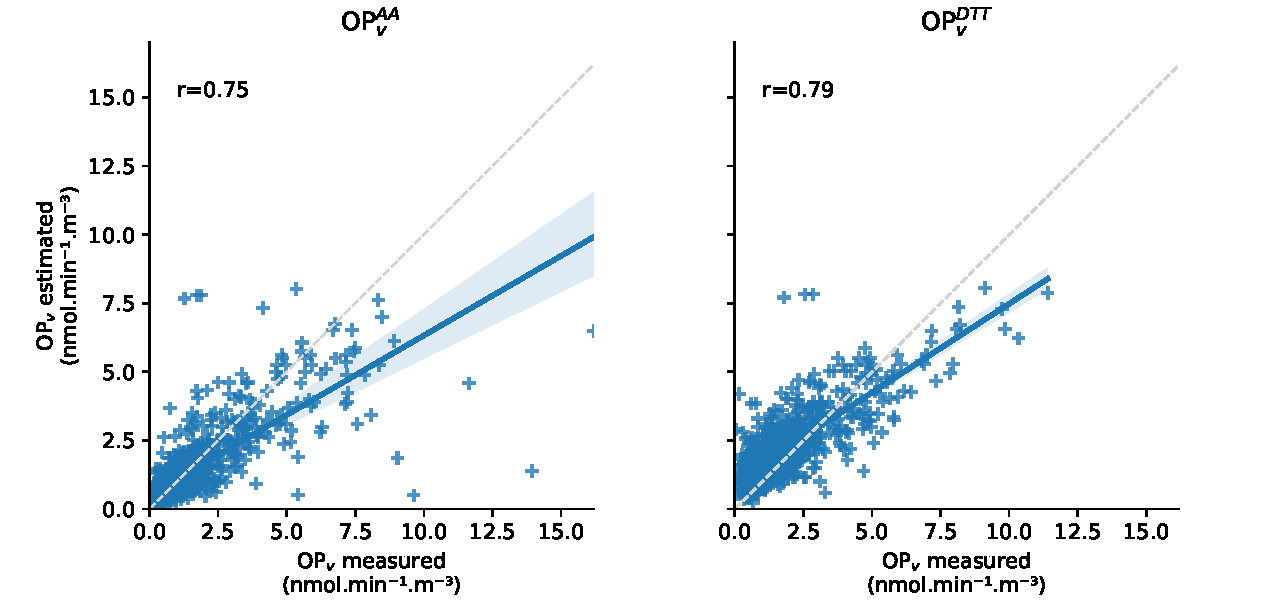
\includegraphics[width=0.8\textwidth]{figures/chapter05/OPGRE-fr_estimated_scatter.pdf}
    \caption{\POAAv{} et \PODTTv{} estimés et mesurés sur le site de GRE-fr depuis 2012.}
    \label{fig:OPGRE-fr-estimated_scatter}
\end{figure}

\paragraph{Importance de l'échantillonage et de l'exposition chronique}%
\label{par:importance_de_l_échantillonage_et_de_l_exposition_chronique}

% Puisque l'approximation reconstruit relativement bien les observations, l'estimation du PO
% les jours non mesurés peut donc être considérée comme acceptable. Ainsi, l'estimation de
% la contribution des sources au PO sur le site de GRE-fr peut se faire en prenant en compte
% l'intégralité de la série de mesure d'Atmo AURA et non plus un échantillon tous les trois
% jours. Le biais de selection dû à la fréquence d'échantillonnage est donc ainsi amoindri.

Les contributions des sources de PO d'après les mesures journalières d'Atmo AURA sur la
station de GRE-fr sont présentées figure~\ref{fig:OPGRE-fr_source_estimated}. % et détaillées dans le tableau~\ref{tab:OPGRE-fr_source_estimated}.
Si elle n'apprend rien de bien nouveau, cette méthode d'estimation certes grossière,
permet la prise en compte d'un très grand nombre de jours d'observation et met d'autant
mieux en lumière la différence entre contribution moyenne et contribution médiane des
sources de \PMdix{} aux différents tests de PO et l'importance de la prise en compte de
l'exposition chronique.

En effet, de par l'importance du PO intrinsèque de la source combustion de biomasse
(\textit{Biomass burning} dans le graphique), sa contribution moyenne annuelle est
importante, notamment pour le \POAAv.  Puisque l'on dispose de
l'ensemble des jours de mesures et que cette source présente une dynamique très
saisonnière, l'écart entre contributions moyenne et médiane est cependant très important.
En revanche, conformément aux POs intrinsèques élevés de la source trafic primaire
(\textit{Road traffic} dans le graphique) et de sa contribution relativement homogène tout au
long de l'année, cette source est la première contributrice au \PODTTv, aussi bien en
moyenne qu'en médiane et l'écart en contribution moyenne et médiane est relativement
faible.

\begin{figure}[ht]
    \centering
    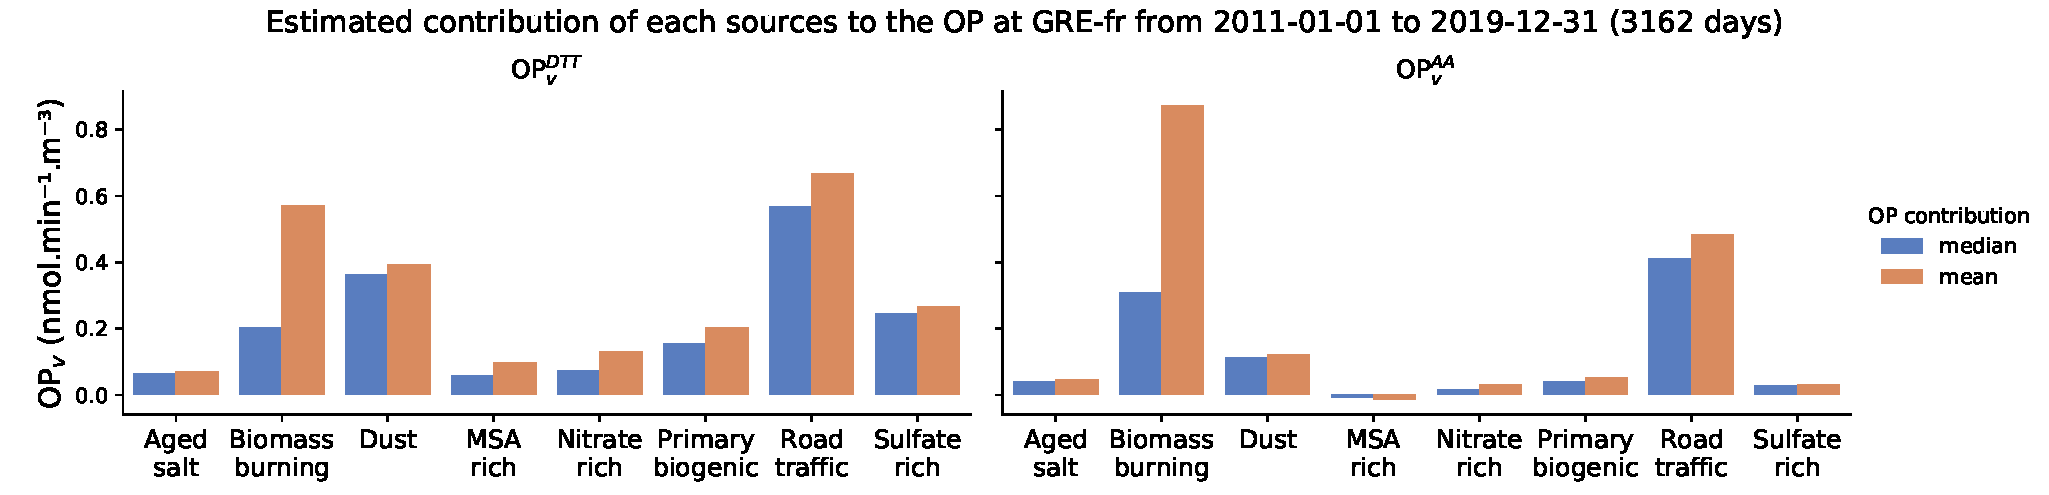
\includegraphics[width=1.0\linewidth]{figures/chapter05/OPGRE-fr_source_estimated.pdf}
    \caption{Contributions estimées moyennes et médianes des sources de \PMdix{} aux
        \PODTTv{} et \POAAv{} sur le site de Grenoble Les Frènes entre 2011 et 2019.}%
    \label{fig:OPGRE-fr_source_estimated}
\end{figure}

% \begin{table}[ht]
%     \centering
%     \footnotesize
%     \begin{tabular}{cp{1cm}p{1.3cm}p{1.3cm}p{1.3cm}p{1.3cm}p{1.3cm}p{1.3cm}p{1.3cm}p{1.3cm}p{1.3cm}}
%         \toprule
%         & & \multicolumn{8}{c}{Estimated source contribution to OP in \si{\opv}}\\
%
%                        &      & Aged salt & Biomass burning & Dust  & MSA rich & Nitrate rich & Primary biogenic & Road traffic & Sulfate rich\\\midrule
%
% \multirow{6}{*}{AAv}   & mean & 0.045 & 0.871 & 0.121 & -0.014 & 0.030 & 0.051 & 0.482 & 0.031\\
%                        & std  & 0.023 & 1.178 & 0.066 & 0.014  & 0.032 & 0.038 & 0.285 & 0.017\\
%                        & min  & 0.002 & 0.008 & 0.005 & -0.114 & 0.001 & 0.001 & 0.041 & 0.001\\
%                        & 25\% & 0.028 & 0.066 & 0.074 & -0.020 & 0.007 & 0.021 & 0.275 & 0.019\\
%                        & 50\% & 0.041 & 0.308 & 0.111 & -0.008 & 0.016 & 0.038 & 0.409 & 0.028\\
%                        & 75\% & 0.058 & 1.265 & 0.158 & -0.004 & 0.042 & 0.072 & 0.626 & 0.041\\
%                        & max  & 0.167 & 6.347 & 0.502 & -0.000 & 0.259 & 0.235 & 1.867 & 0.138\\
%                           \midrule
%  \multirow{6}{*}{DTTv} & mean & 0.070 & 0.571 & 0.392 & 0.096 & 0.131 & 0.202 & 0.668 & 0.266\\
%                        & std  & 0.036 & 0.772 & 0.214 & 0.096 & 0.142 & 0.153 & 0.395 & 0.145\\
%                        & min  & 0.003 & 0.005 & 0.016 & 0.001 & 0.004 & 0.006 & 0.057 & 0.013\\
%                        & 25\% & 0.043 & 0.043 & 0.239 & 0.027 & 0.033 & 0.084 & 0.382 & 0.162\\
%                        & 50\% & 0.064 & 0.202 & 0.361 & 0.058 & 0.073 & 0.154 & 0.568 & 0.245\\
%                        & 75\% & 0.090 & 0.829 & 0.510 & 0.140 & 0.184 & 0.286 & 0.868 & 0.348\\
%                        & max  & 0.261 & 4.162 & 1.623 & 0.772 & 1.129
%                        & 0.937 & 2.587 & 1.170\\
%                           \bottomrule
%     \end{tabular}
%     \caption{Contributions estimées des sources de PM aux \POAAv{} et \PODTTv{} pour
%     Grenoble Les Frènes entre 2011 et 2019 (n=3162 jours)}
%     \label{tab:OPGRE-fr_source_estimated}
% \end{table}

\bigskip

En définitive, il est également envisageable d'établir une cartographie du PO à partir
soit des mesures satellites de concentration de \PMdix, soit des sorties de modèle CTM.
Cependant, du fait de ses nombreuses hypothèses et limitations, cette première méthode
d'estimation ne peut en revanche pas se substituer à une étude complète de la prévision du
PO par modèle déterministe.
En effet, elle n'est basée que sur des caractéristiques moyennes très générales et il
n'est donc pas possible de prévoir quoi que ce soit en dehors de cette état moyen. Par
exemple, il est impossible d'estimer le PO lors du confinement de 2020 avec cette
méthode, tant l'écart entre la normalitée et cette période est importante.
En introduisant une part de spécificité spatiale et temporelle plus importante, les CTM
peuvent éventuellement apporter une meilleure prévisibilité.

\subsection{Prévision déterministe du PO (modélisation CTM)}

\begin{tcolorbox}[colback=red!5!white,colframe=Melon,title=Note]
    L'utilisation des CTM pour l'étude du PO a commencé grâce à une collaboration avec le
    TNO et une première visite de deux semaines (sur financement de l'IDEX DataInstitute de l'université Grenoble Alpes) lors du
    workshop LOTOS-EUROS de janvier 2019 et constituera le cadre de mon post-doctorat 2021-2022.

    Le même travail a commencé lors du stage et la poursuite en thèse de Matthieu Vida, en
    collaboration IGE-LISA pour le modèle Chimère.

    Un résultat d'ores et déjà très encourageant est déjà soumis utilisant CAMx
    \parencite{daellenbachSourcessubmitted}, pour lequel mon implication a principalement
    porté sur la validation des résultats du modèle.
\end{tcolorbox}

Si la partie précédente proposait une première méthode approchant de façon imparfaite la prévision du PO à partir
du calcul de la masse des \PMdix{} estimée par les CTM, il est certainement
préférable d'inclure directement la variable ``potentiel oxydant'' dans ces modèles.

Cependant, le ``PO'' n'étant pas une espèce chimique évoluant et réagissant dans le temps, son
estimation ne peut se faire que a posteriori et soit (i) à partir du PO intrinsèque de chacune
des espèces chimiques, soit (ii) en estimant la contribution des sources à la masse des \PMdix.
Avec la voie (i), nous retrouvons les mêmes limitations que pour l'inversion par espèce
chimique. Mais pour emprunter la voie (ii), il faut donc
réussir à estimer tout d'abord correctement les sources de \PMdix{} dans les modèles CTM.

Ensuite, deux solutions sont envisageables:
\begin{enumerate}
    \item estimer un PO intrinsèque par source d'émission des CTM en utilisant le même
        procédé que celui développé durant cette thèse en utilisant les mesures de PO à
        différentes stations;
    \item établir une équivalence entre source CTM et facteur PMF, puis appliquer les
        PO intrinsèques des facteurs PMF aux sources estimées par CTM.
\end{enumerate}

La première solution permettrait la prise en compte d'un nombre de sources beaucoup plus
grand que celui retenu dans les PMF (émissions portuaires, différents type de résidentiel
ou trafic, feu de forêt, etc) puisque les sources des CTM sont fondées sur les SNAP, qui
sont très nombreux.
En revanche, cette solution, dans son implémentation actuelle à travers le ``source
labelling'', ne prend en compte uniquement que les sources primaires. Par exemple, la
condensation des \ce{NO_x} du trafic routier et de l'ammoniac de l'agriculture forme du
nitrate-d'ammonium et est attribué selon une moyenne pondérée aux sources trafic et
agricole. Il y a donc une perte d'information entre sources primaire et secondaire.

La deuxième solution nécessite une comparaison des émissions chimiques considérées dans
chacun des SNAP utilisés avec les profils chimiques des facteurs PMF. S'il est possible
d'établir un rapprochement entre ces deux nomenclatures, il sera possible d'estimer le PO
apporté par ces sources.

Dans les deux cas, le développement de la technique de ``source-labelling'' et la base de
données unique d'attribution des sources en site récepteur appellent à une étude de
sensibilité des prédictions des CTM. Notamment, LOTOS-EUROS\footnote{LOTOS-EUROS:
    \url{https://lotos-euros.tno.nl/}} (abrégé LE) développé au TNO (\textit{Netherlands Organisation for
Applied Scientific Research}) a récemment rendu disponible cette technique à travers TOPAS\footnote{TOPAS:
TNO Operational Pollution Apportionment Service (\url{https://topas.tno.nl/})}. Cette
avancée est possible grâce à l'implémentation de la méthode de \cite{kranenburgSource2013} dans
LOTOS-EUROS v2 \autocite{mandersCurriculum2017}.

Une collaboration entre l'IGE et le TNO a donc été engagée afin de confronter les
prédictions de LE aux sorties PMF. Aussi, lors de mon séjour au TNO en 2018, nous
avons pu apporter une preuve de concept de la faisabilité de la prédiction du PO par
LE pour deux sources chimiquement proches entre LE et les PMF.
La figure~\ref{fig:OPmap} présente pour le 10 février 2017 à 11h30 la contribution du
transport routier et de la combustion résidentielle à la masse et au \PODTTv{} pour
l'ensemble de l'Europe (figure issue d'un run d'un mois destinée à l'étude d'un pic de
pollution).

Ce travail, très préliminaire, se poursuivra après ma thèse dans le cadre de cette
collaboration entre l'IGE et le TNO.

\begin{figure}[ht]
    \centering
    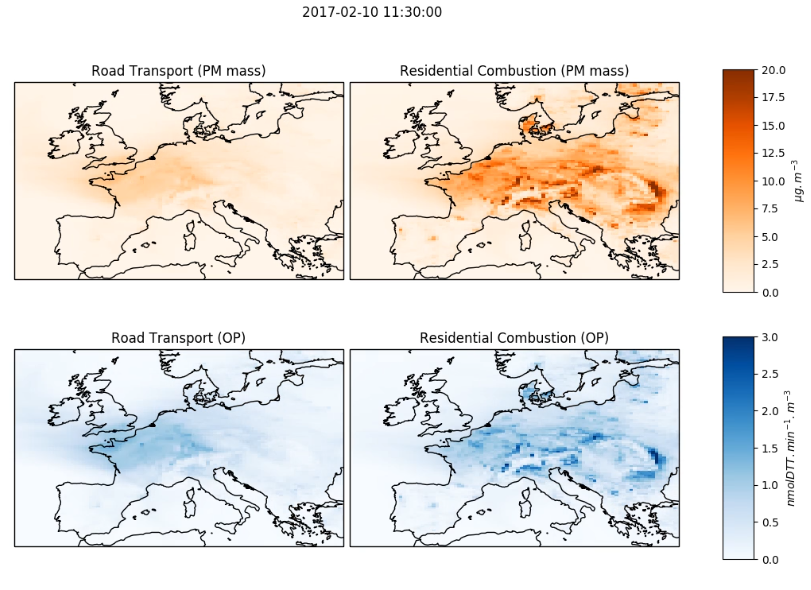
\includegraphics[width=0.8\linewidth]{figures/chapter05/OPmap.png}
    \caption{Preuve de concept de la modélisation grande échelle du potentiel oxydant,
    utilisant le \PODTT{} intrinsèque du trafic routier et de la combustion de biomasse
estimée par \cite{weberSourceinprep.} appliqué aux prévisions de LOTOS-EUROS.}%
    \label{fig:OPmap}
\end{figure}

Cette preuve de concept en 2018 a intéressé les développeurs
d'un autre modèle de chimie transport: Chimère. La
même technique de ``source-labelling'' a été implémentée dans Chimère courant 2020, et un
travail identique à celui entamé avec le TNO
et LE sur le confrontation des résultats de contribution des sources pour des sites
spécifiques est en cours avec le LISA et Chimère. Notamment, de février à juillet 2020, le
stage de M2 de Matthieu Vida (LISA/IGE) portait sur cette thématique, qu'il va poursuivre en thèse à
la rentrée universitaire 2020 (thèse ADEME/Dim Qi2, co-encadrement LISA/IGE).

Parallèlement, \cite{daellenbachSourcessubmitted} ont conduit une étude similaire à celle
de \cite{weberSourceinprep.}, mais n'incluant que 109 mesures composites de potentiel
oxydant sur 6 sites de prélèvement en Suisse. Dans cette étude, à laquelle j'ai pris
part, le couplage entre PO intrinsèque et sources déterminées par le CTM CAMx est proposé.
Les résultats obtenus montrent une fois de plus
l'importance de la combustion de biomasse mais aussi de la source trafic routier dans
les zones densément peuplées. En estimant l'exposition des populations avec soit la masse de
\PMdix{} soit la quantité de \POv{} inhalée, cette étude montre une
redistribution complète de l'importance des sources entre concentrations massiques et
potentiels oxydants. Encore une fois, l'importance du trafic routier s'accroît
considérablement et l'aérosol inorganique, pourtant dominant en terme de masse, n'a plus
qu'une influence minime sur l'exposition aux \POv.

Le même type d'étude, fondé sur une représentativité spatiale et temporelle des données
d'entrée plus importante à l'échelle européenne devra être généralisé dans le futur.

% \begin{figure}[ht]
%     \centering
%     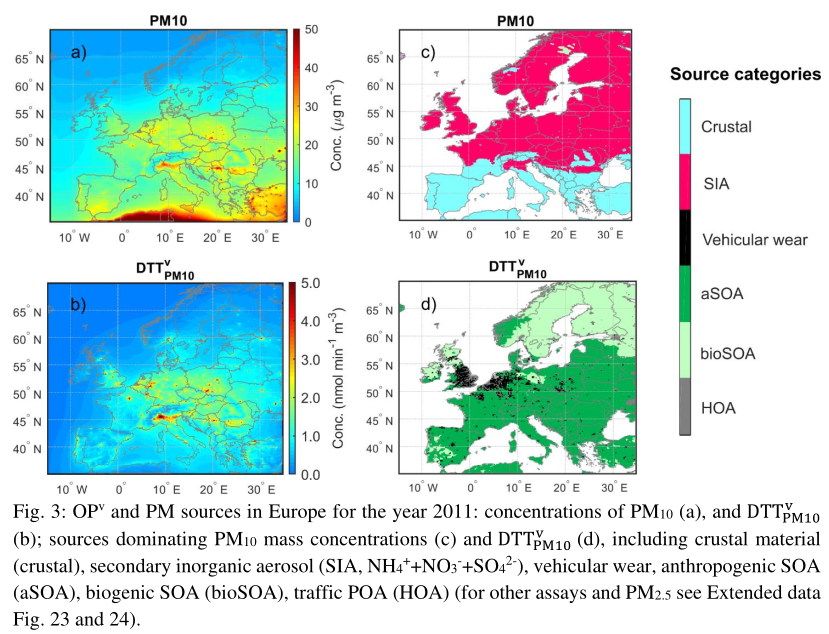
\includegraphics[width=0.8\linewidth]{figures/chapter05/map_kaspard.png}
%     \caption{Estimation européenne du \PODTTv{} et des sources associées par
%     \cite{daellenbachSourcessubmitted}.}%
%     \label{fig:map_kaspard}
% \end{figure}

\section{Contribution non linéarité des sources aux PO : réseaux de neurone}%
\label{sec:reseau_neurone}

\begin{tcolorbox}[colback=red!5!white,colframe=Melon,title=Note]
    Cette partie reprend les travaux préliminaires présentés par \cite{borlazaUrbaninprep.} sur 
    l'attribution du PO aux sources d'émissions sur trois sites Grenoblois. Le stage de M2 de
    \cite{fichesMachine2020}, que j'ai encadré, s'est également attaché à la mise en place et
    l'interprétabilité des réseaux de neurones dans une optique d'attribution des sources
    de potentiel oxydant des particules atmosphériques.
\end{tcolorbox}

\subsection{Limitations inhérentes aux modèles linéaires}%
\label{sub:limitations_inhérentes_aux_modèles_linéaires}


Il est maintenant établi que la mesure du PO n'est pas linéaire avec la concentration des composés
chimiques. Il est donc logique de dire qu'il en est de même avec la contribution des
sources.
Or, jusqu'à présent, le PO des sources de PM a été estimé à partir d'un modèle linéaire,
que ce soit par introduction du \POv{} dans une PMF, par régression linéaire multiple ou
par ACP.
De plus, aucun terme d'interaction entre sources n'est pris en compte alors même que
le potentiel ``effet cocktail'' entre composés chimiques sur le PO est documenté, comme le
montre la figure~\ref{fig:charrier_hydrogen_2014_fig4} issue de
\cite{charrierHydrogen2014} ou encore 
\cites[figure S7 du supplément]{charrierDithiothreitol2012}{xiongRethinking2017}{samakeUnexpected2017}{yuSynergistic2018}
(à noter également que récemment, \cite{gaoCharacterization2020} ont introduit des
potentielles interractions entre metaux et matières organiques et Fer-Cuivre lors d'une régression PO
versus chimie et des effets synergiques sont bien observés).

\begin{figure}[ht]
    \centering
    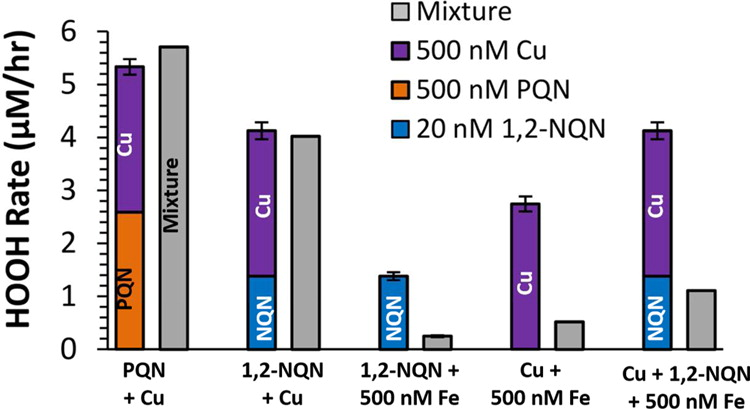
\includegraphics[width=0.5\linewidth]{figures/chapter05/charrier_hydrogen_2014_fig4.jpg}
    \caption[Effets synergétiques entre métaux et quinones sur le PO]{Effets
        synergétiques entre métaux et quinones sur le PO. \cite[figure 4]{charrierHydrogen2014}: Initial rates of HOOH production in
    laboratory mixtures of quinones and/or transition metals (gray bars) compared to the
    sum of the rates from the individual redox-active species (stacked colored bars). Error
    bars of the colored stacked bars are the propagated errors of the sum (all have replicate
    samples). The concentrations of metals and quinones are constant: Cu, Fe, and PQN are at
    500 nM, and 1,2-NQN is at 20 nM.}%
    \label{fig:charrier_hydrogen_2014_fig4}
\end{figure}

Si ces modèles linéaires permettent une première estimation de la contribution des sources et sont
facilement interprétables, ils présentent donc, par construction, deux biais majeurs: non
prise en compte des effets d'interaction entre sources et non prise en compte de la non
linéarité du PO.

L'ajout de terme d'interaction sous forme de produit des concentrations de sources serait
une solution pour estimer le premier biais -- bien que les différentes interactions soit en grande partie inconnues --
% (oui mais sur quelle base en pratique on arriverait à définir ce terme d'interaction? à partir d'expériences type charrier au dessus ou alors comme on a fait dans Samake sur le po des bioarérsols, mais dans ce cas on serait vite limité car impossible de faire toutes les expériences) 
mais le deuxième biais ne peut tout simplement
pas s'estimer par un modèle linéaire. Aussi, l'ajout de termes non linéaires n'est pas
évident car il semble exister une grande diversité de réponses non linéaires selon les
espèces chimiques
considérées~\autocite{charrierDithiothreitol2012,charrierBias2016,calasImportance2017}

Par conséquent, il convient de construire un modèle présentant les caractéristiques
suivantes :
\begin{itemize}
    \item prise en compte de la non-linéarité de la dose-réponse de la concentration des
        sources,
    \item prise en compte d'effets conjoints, potentiellement non linéaires et négatifs,
        entres les sources,
    \item sans connaissance a priori des relations dose-réponse ou entre sources.
\end{itemize}

\subsection{Les réseaux de neurones}%
\label{sub:les_réseaux_de_neurones}

Les réseaux de neurones artificiels (\textit{artificial neural network} ANN) semblent être
un type de modèle répondant à ces critères. Ils sont plus complexes et flexibles que les
modèles linéaires, et sont connus pour être capables de prendre en compte des phénomènes
fortement non linéaires. Aussi, leurs capacités à apprendre des relations complexes et ce
sans aucune connaissance a priori, simplement en s'entraînant sur un ensemble de données
suffisant, en font un outil très intéressant.
Ce type de modèle a été appliqué avec succès en prévision de la qualité de l'air pour le
\ce{NO2} et les \PMdix{} par~\cite{kukkonenExtensive2003} en comparaison à un modèle
linéaire et déterministe. Dans d'autres disciplines des sciences de l'environnement, ce
type de modèle a également montré son intérêt pour l'évaluation de la qualité de
l'eau~\autocite{nathanApplication2017}.

\subsubsection{Présentation succincte d'un réseau de neurone}%
\label{ssub:présentation_succincte_d_un_réseau_de_neurone}


Formellement, un réseau de neurones est un graphe orienté pondéré, où lorsque deux
nœuds (ou neurones) sont connectés (i.e lié par un bord orienté du graphe), le résultat en
sortie du neurone devant est utilisé comment entrée du neurone de derrière.
Autrement dit un réseau de neurones consiste en une succession de ``nœuds'' (ou synapses, ou
neurones) connectés entres eux par des relations linéaires appelées ``poids''. Le principe
mime un réseau de neurones biologiques naturels très simpliste où chacune des
informations reçue par un neurone se propage à d'autres neurones afin de prédire une
valeur finale (par ex. le \POv) en fonction d'un signal initial (par ex. la
concentration massique des sources de PM).
On distingue trois types de neurones:
\begin{itemize}
    \item neurones d'entré (input) (connectés aux variables d'entrées),
    \item neurones de sortie (output),
    \item neurones cachés (répartis en une ou plusieurs couches).
\end{itemize}
Le plus couramment utilisé est le \textit{Multi Layer Perceptron} (MLP), qui est un
réseau a-cyclique où les neurones sont structurés en couches successives\footnote{Il est
d'ailleurs montré que le MLP est un approximateur universel.}, illustré dans la
figure~\ref{fig:MLP_architecture}.

\begin{figure}[ht]
    \centering
    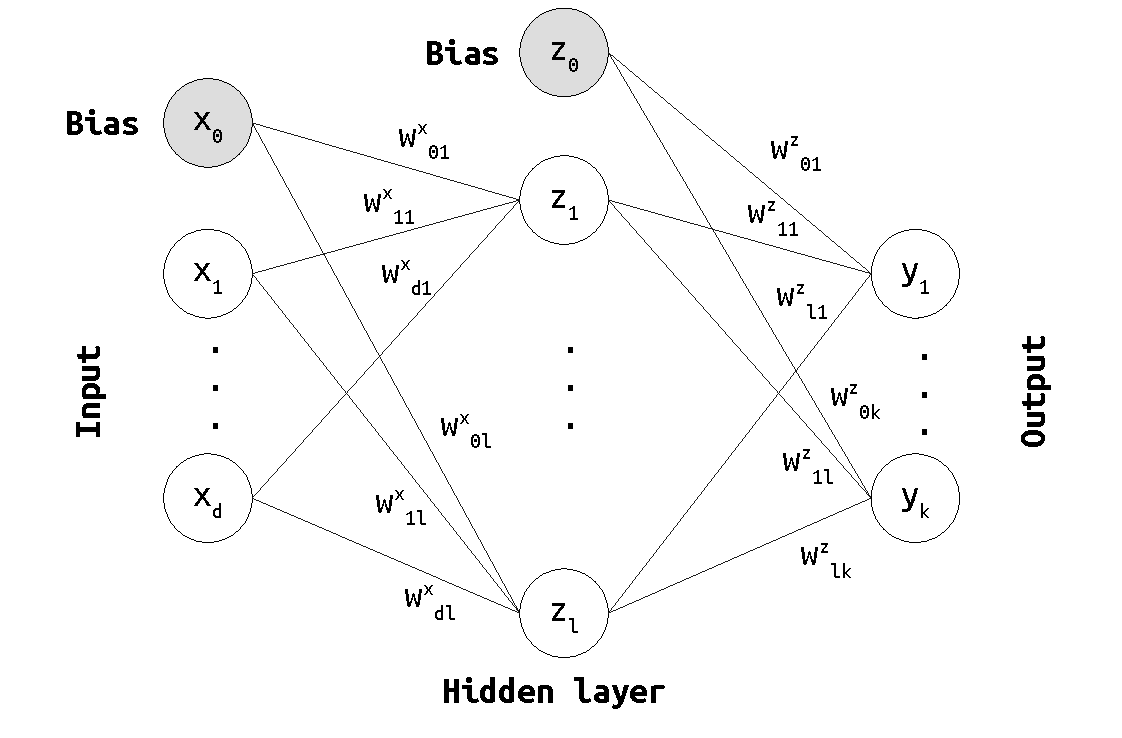
\includegraphics[width=0.7\linewidth]{figures/chapter05/MLP_architecture.pdf}
    \caption[Architecture simplifée d'un MLP à une couche cachée]{Architecture d'un MLP à une couche cachée, $d$ neurones d'entrée, $l$
    neurones sur la couche cachée et $k$ neurones de sortie (notation d-l-k). $x$
    représente la valeur des variables explicatives (par ex. la concentration massique des
    sources de \PMdix) et $y$ la variable prédite (par ex. le \POAAv{} et \PODTTv).}%
    \label{fig:MLP_architecture}
\end{figure}

Au sein de chaque nœud, l'information reçue est condensée en une valeur unique puis propagée à
son tour aux neurones suivants. En prenant l'exemple du MLP décrit par la
figure~\ref{fig:MLP_architecture}, cette condensation d'informations pour la première
couche se fait selon l'Eq.~\ref{eq:ANN_neurone}:
\begin{align}
    \label{eq:ANN_neurone}
    \forall j \in \{1, ..., l\}, z_j &= H\left( \sum_{i=1}^d w^x_{i,j} \times x_i + w^x_{0,j} \right)
\end{align}
avec $w^x_{i,j}$ les poids entre les neurones des couches d'entrée et cachée, et
$w^x_{0,j}$ une constante d'activation pour le neurone $j$. La fonction $H$
peut-être de différents types, mais est très souvent non-linéraire. Le fait de combiner
deux
couches de neurones et d'ajouter une fonction d'activation non linéaire amène la
complexité recherchée permettant la prise en compte des phénomènes complexes.

Chacun des poids $w$ est inconnu a priori. Ils sont estimés par processus itératif et
rétro-propagation à partir d'un ensemble de données d'entraînement pour lesquelles les
valeurs d'entrées et de sorties sont connues. Les poids sont donc ``appris'' -- d'où le
terme de \textit{machine learning} -- par minimisation d'une fonction coût entre prédictions
et observations (de manière similaire à l'algorithme PMF).

En revanche, du fait de leurs complexités, même si les prédictions se trouvent être
correctes, il peut être compliqué d'interpréter le modèle obtenu.


Dans le cadre d'un financement du projet Idex DataInstitute de l'Université Grenoble Alpes, j'ai
obtenu un financement pour l'encadrement d'un stagiaire de M2, Jean-Baptiste Fiches, afin
de travailler spécifiquement sur ces questions :
\begin{enumerate}
    \item Est-il possible d'appliquer un réseau de neurones pour la prédiction du potentiel
        oxydant ?
    \item Ces réseaux présentent-ils des performances statistiques meilleures que la
        régression linéaire ?
    \item Est-ce que la non-linéarité attendue est bien observée ?
    \item Comment interpréter ces modèles pour retrouver une information géochimique (i.e.
        PO des différentes sources de PM) ?
\end{enumerate}
Ce travail s'incorporera prochainement dans l'étude de \cite{borlazaUrbaninprep.} du
projet Mobil'Air, afin de comparer les sources de potentiels oxydants sur la
métropole Grenobloise estimées par régression linéaire multiple (MLR) et réseau de
neurones artificiel (MLP).


\subsubsection{Résultats préliminaires}%
\label{ssub:résultats_préliminaires}

\paragraph{Performance statistique}%
\label{par:performance_statistique}

Appliqués sur les trois sites de la métropole Grenobloise, le MLP a été entraîné sur
\SI{80}{\percent} des données et testé sur les \SI{20}{\percent} restant. Le MLR a quant à
lui été entrainé sur l'ensemble des séries de mesures\footnote{Une comparaison pour les mêmes
ensembles d'entrainement et de test est en cours.}.
Les performances statistiques de la prediction des MLP sont du même ordre que celles
obtenues pour le MLR alors même que le MLP n'a pas été entrainé sur ces données (figure~\ref{fig:perfMLPMLR}).
Ainsi, le MLP prédit aussi bien chaque \POv{}
(mesuré par AA, DTT et DCFH) sur les trois sites que l'explique le MLR.
Ce type de modèle permet donc d'expliquer au moins aussi bien que le MLR les PO à partir
des sources d'émissions de \PMdix.

\begin{figure}[ht]
    \centering
    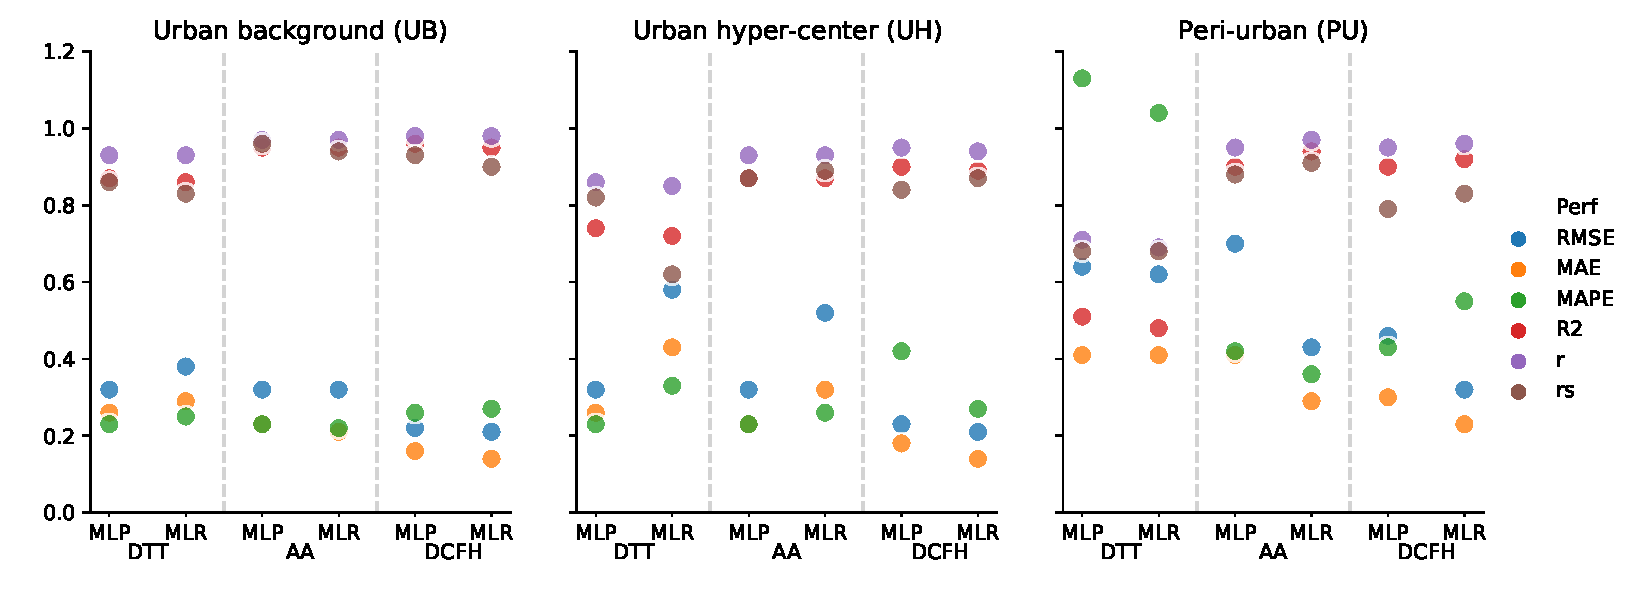
\includegraphics[width=1.0\linewidth]{figures/chapter05/perfMLPMLR.pdf}
    \caption{Performances statistiques des prédictions du modèle MLR et MLP sur les 3
    sites de Grenoble \autocite{borlazaUrbaninprep.}. (UB = GRE-fr, UH = GRE-cb, PU = Vif)}%
    \label{fig:perfMLPMLR}
\end{figure}


\paragraph{Présence d'effets non linéaires}%
\label{par:présence_d_effets_non_linéaires}

Pour estimer si le MLP capture bien des relations non-linéaires, deux expériences sont
menées.  Dans les deux cas, le MLP est entraîné sur le jeu de données du site de GRE-fr.
Deux situations fictives sont ensuite imaginées.

La première consiste à estimer le \PODTTv{} par le MLP, toutes contributions des sources
nulles sauf une, variant de 0 à 24~\si{\ugm}. La réponse du \PODTTv{} en fonction de
l'augmentation linéaire de la contribution de chacune des sources est présentée
figure~\ref{fig:figures/chapter05/10sourcesLinearite}. On y observe bien une réponse
non-linéaire en fonction d'une augmentation linéaire de la contribution de
chaque source. On note par ailleurs dans ce modèle un biais constant de l'ordre de
\SI{-0.5}{\opv} lorsqu'aucune source n'est présente.
On remarque également l'influence négative des sources primaires biogéniques, nitrate-rich
et MSA-rich (i.e Marine SOA dans la figure) mais aussi la forte influence des sources
trafic primaire et industrielle.

\begin{figure}[ht]
    \centering
    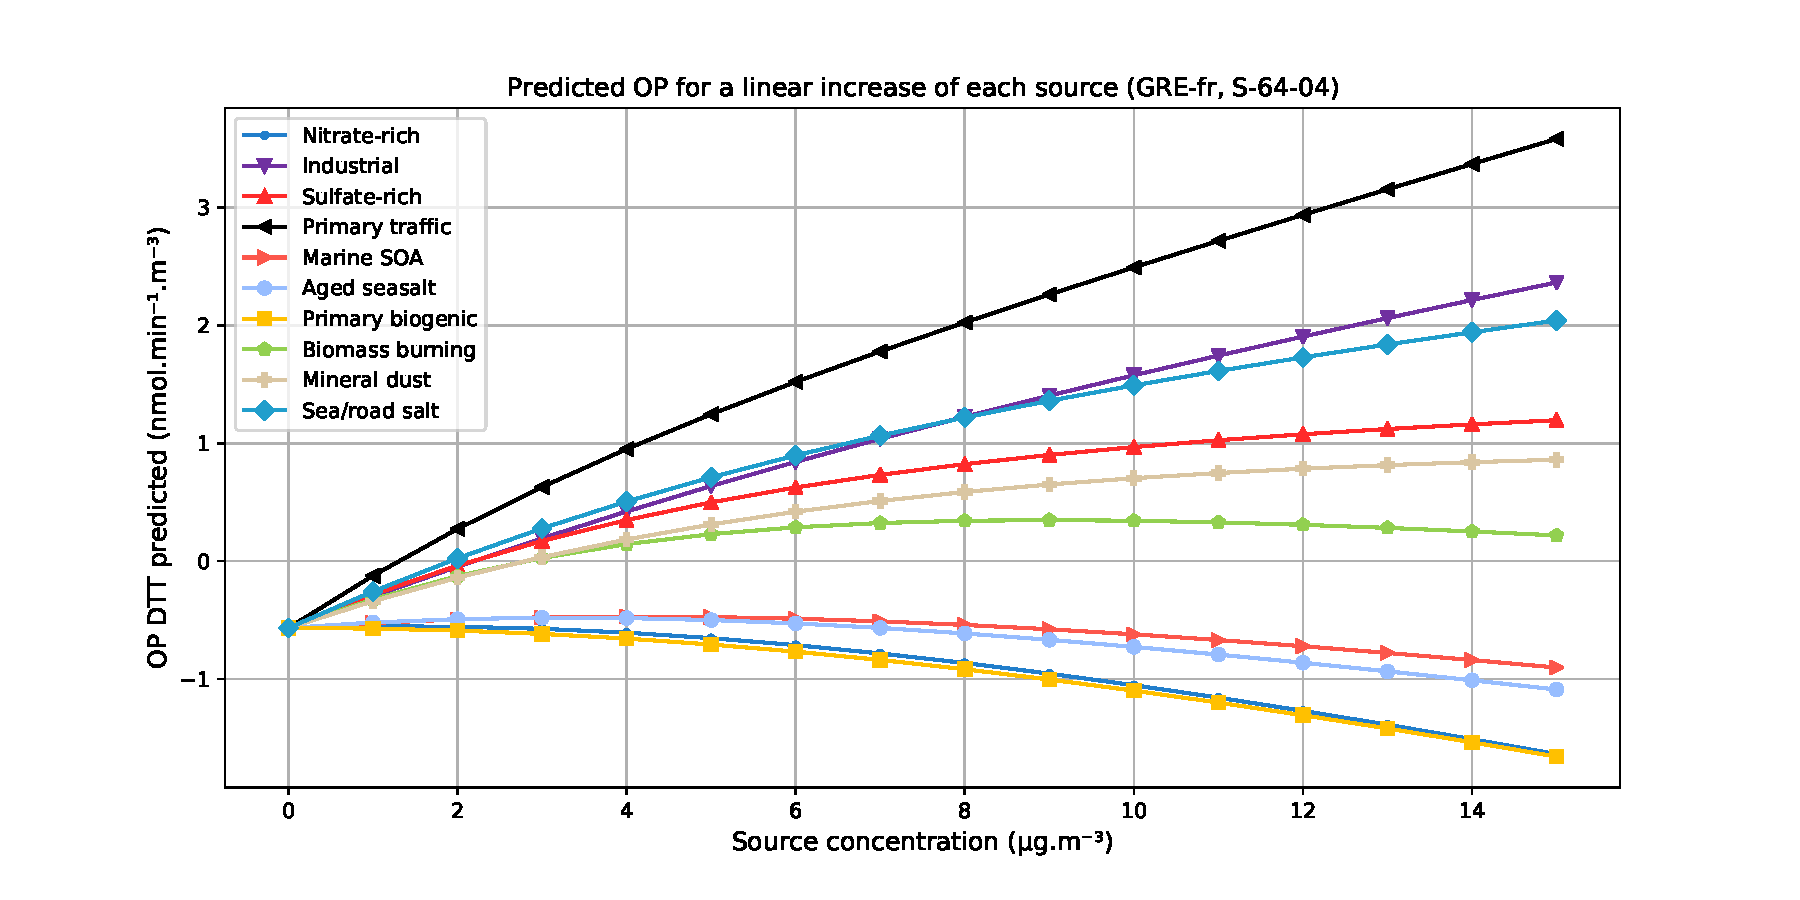
\includegraphics[width=0.9\linewidth]{figures/chapter05/prediction_other_0_softplus-64-0.4.pdf}
    \caption{Effet non linéaire de l'augmentation de la concentration d'une source
        d'émission sur le \PODTTv{} d'après un réseau de neurones entraîné sur GRE-fr. Source: \cite{fichesMachine2020}.}%
    \label{fig:figures/chapter05/10sourcesLinearite}
\end{figure}

Dans la deuxième situation, on cherche à estimer si le MLP prévoit des effets non-additifs
lors de la présence conjointe de plusieurs sources de \PMdix. L'expérience prédit donc le
\PODTTv{} pour un ensemble d'échantillons de test où cette fois deux sources présentent des
concentrations variant chacune de 0 à \SI{15}{\ugm}.
Si l'effet est additif, le gradient de l'augmentation du \PODTTv{} dans un espace en
deux dimensions représentant la contribution de chacune des sources est sensé être
linéaire.
Dans le cas contraire, cela indiquera un effet cocktail entre ces deux sources.
La figure~\ref{fig:figures/chapter05/coktail_Primary traffic_Nitrate-rich} montre
l'influence de la présence conjointe de deux sources d'émissions (\textit{Primary traffic}
et \textit{Nitrate-rich}) sur le \PODTTv. L'effet conjoint est bien non linéaire car alors
que le \textit{Nitrate-rich} seul tend à diminuer le \PODTTv, une augmentation du PO est
observé lors de la présence conjointe avec la source \textit{Primary traffic}. Dans la gamme de
concentration réaliste étudiée, la présence de \textit{Nitrate-rich} diminue le \PODTTv{}
pour des concentrations du \textit{Primary traffic} inférieures à \SI{4}{\ugm}, mais
augmente puis diminue le \PODTTv{} lorsque la concentration de \textit{Primary traffic} est
supérieure à \SI{5}{\ugm} et un maximum est obtenu pour des valeurs des contributions du
\textit{Primary traffic} de \SI{15}{\ugm} et du \textit{Nitrate-rich} de \SI{6}{\ugm}.

\begin{figure}[ht]
    \centering
    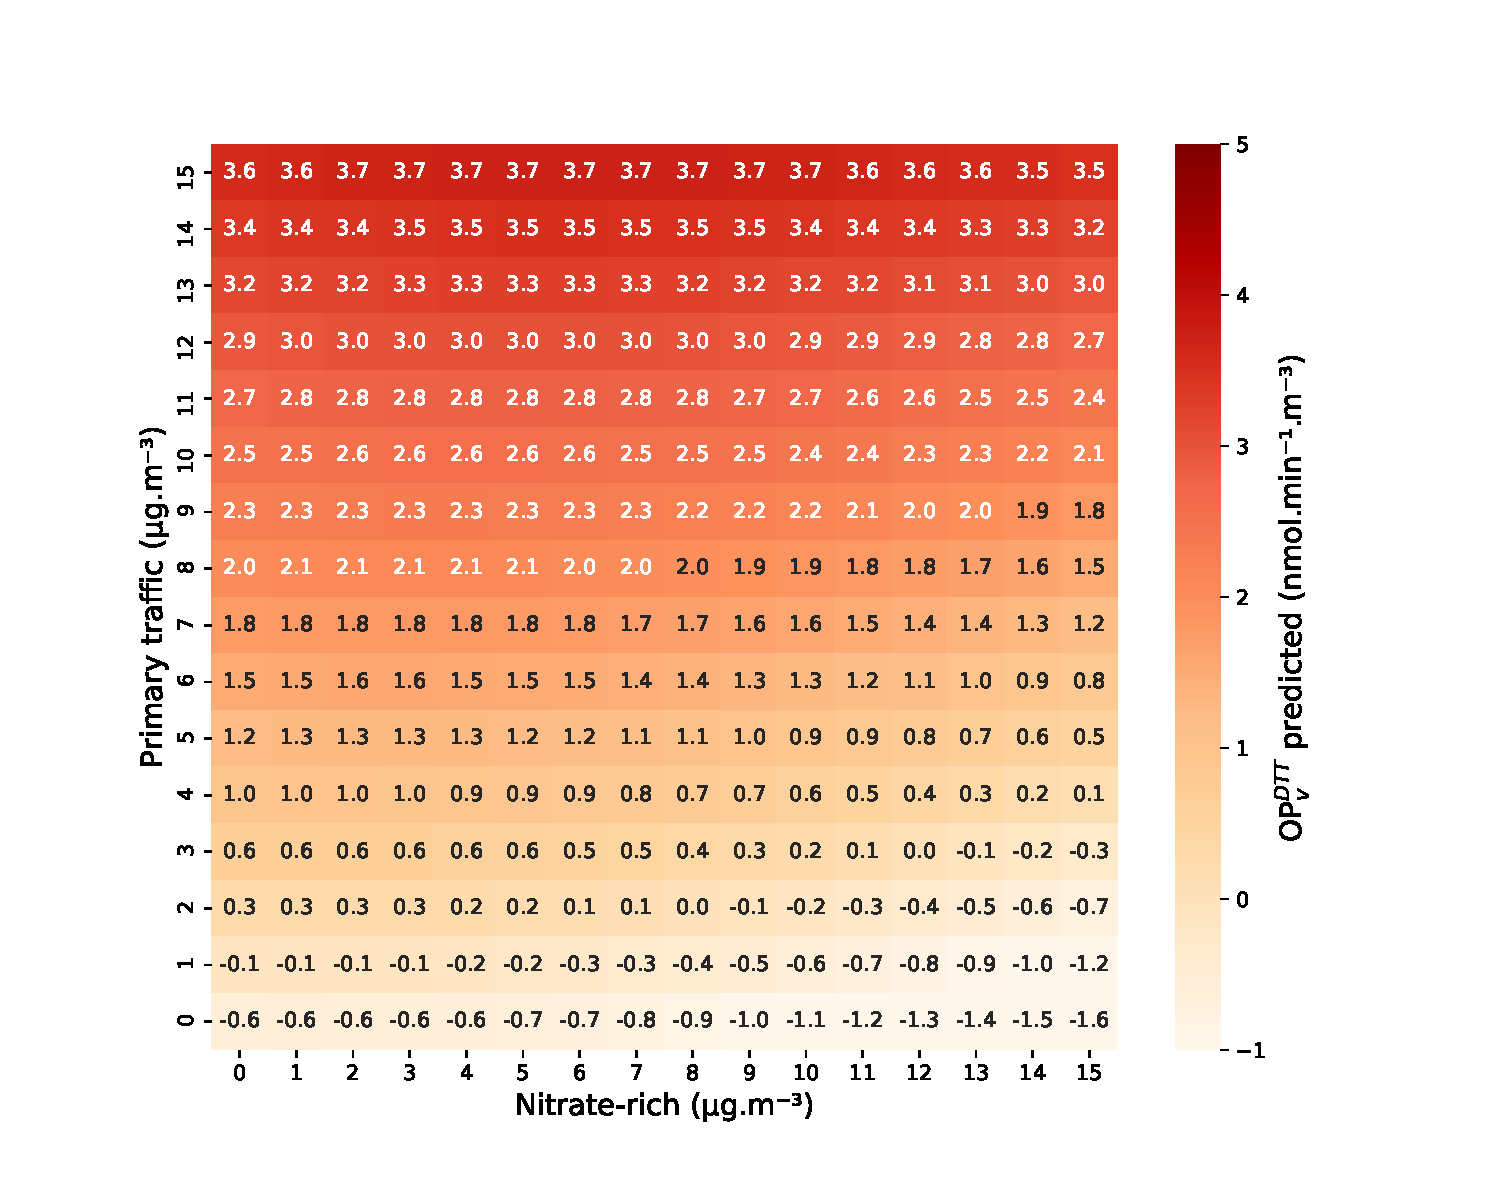
\includegraphics[width=0.7\linewidth]{figures/chapter05/coktail_Primary traffic_Nitrate-rich.pdf}
    \caption{Effet synergétique non-linéaire sur le \PODTTv{} entre la source \textit{Primary
    traffic} et \textit{Nitrate-rich} sur le site de GRE-fr.}%
    \label{fig:figures/chapter05/coktail_Primary traffic_Nitrate-rich}
\end{figure}

\paragraph{Contribution des sources au PO}%
\label{par:contribution_des_sources_au_po}

Enfin, il se pose la question de l'estimation de la contribution des sources aux PO. Du
fait de la complexité du modèle, il n'est pas possible d'attribuer \emph{un} PO
intrinsèque par source, celui-ci étant changeant en fonction d'autres paramètres.
La technique utilisée est donc similaire à celle présentée
en~\ref{par:source_apportionment} dite de \textit{brute-force} pour les CTM. À une
simulation de référence pour laquelle toutes les sources sont prises en compte est
soustrait les résultats de différentes simulations où une source est mise artificiellement à une
contribution nulle.  La différence nous apprend donc quel aurait été le \POv{} en
l'absence de chacune des sources.
Cette technique permet donc de répondre à la question
\begin{quote}
   Si les émissions de cette source sont diminuées ou supprimées, quels impacts cela va-t-il
   avoir sur le \POv{} final ?
\end{quote}
mais ne répond en revanche pas à
\begin{quote}
   Dans la concentration ambiante de PM, à combien s'estime la contribution de cette source
   d'émission ?
\end{quote}

Ces différentes voies sont actuellement explorées au sein du stage de Jean-Baptiste Fiches
que j'encadre et seront éventuellement présentés dans \cite{borlazaUrbaninprep.}.

\section{Vers l'exposition fine et les impacts épidémiologiques du PO}

Comme rappelé en introduction du chapitre, la mesure du PO et son application comme outil
de mesure de la qualité de l'air demande nécessairement des études sur la capacité
prédictive des différents tests de PO sur les impacts sanitaires.
Aussi, dans le mode de vie occidental, nous passons le plus clair de notre temps en espace
clos intérieur (domicile ou travail
principalement)~\autocite{netheryTime2009,ouidirEstimation2015}. La qualité de l'air
mesurée dans les stations conventionnelles en air extérieur des réseaux de surveillance
n'est donc peut-être pas représentative de l'exposition réelle des
individus~\autocite{sauvainOxidative2015}.

Dans le cadre du project IDEX Mobil'Air interdisciplinaire de l'UGA, la mesure de qualité
de l'air extérieur avant et après la mise en place d'une zone à faible émission dans la
métropole est couplée à des mesures d'expositions personnelles et à des mesures en air intérieur. Les mesures
d'exposition personnelles sont similaires à celles l'étude pilote de \cite{ouidirEstimation2015}
portant sur l'exposition personnelle de 40 femmes enceintes, mais grandement étendues (projet
SEPAGES~\autocite{lyon-caenDeciphering2019}). La cohorte SEPAGES, coordonnée à l'IAB par l'équipe d'épidémiologie environnementale (PI R. Slama) a pour ambition la mesure d'un très large
ensemble de marqueurs phénotypiques pour un corpus d'environ 480 couples mères-enfants
suivis pendant la grossesse et les premières années des enfants. Parallèlement,
l'exposôme est mesuré très finement, prenant en compte l'exposition personnelle des
sujets dès le premier trimestre de la grossesse grâce au port de micro-capteurs autonomes.

La collaboration entre les équipes de l'IAB et l'IGE au sein du projet Mobil'Air permettra la mesure de l'exposition personnelle
du PO, en plus de celle au \ce{NO2} et à la masse des \PMdc{} au sein de la cohorte SEPAGES. Les faibles masses prélevées
ont nécessité une adaptation méthodologique sur la mesure du PO afin de réduire les
seuils de quantification de ces tests.
L'exposition intérieure des foyers est également quantifiée avec des mesures de la chimie des PM et de leur PO.

Cette collaboration nous permet une caractérisation précise de
l'exposition personnelle maternelle en lien avec un ensemble conséquent de variables
phénotypiques du nouveau-né.
De façon similaire à l'étude de \cite{ouidirEstimation2015}, l'effet de l'exposition au
\ce{NO2}, concentration massique des \PMdc{} mais surtout aux \POAAv{} et \PODTTv{} est en
cours de publication par \cite{borlazaPersonalinprep.}.
Grâce à cette étude, le pouvoir prédictif comparé de la métrique de la masse ou du PO des \PMdc{}
sur le petit poids de naissance ou la circonférence crânienne, parmi d'autres variables,
pourra être évalué.

Finalement, afin d'augmenter la résolution spatiale nécessaire aux prévisions
épidémiologiques, la thèse d'Anouk Marshal (financement ADEME/ANSES, co-encadrement
IGE/IAB) débutant à l'automne 2020 à
l'IGE aura pour objectif d'établir un modèle de \textit{land use regression} (LUR) sur
Grenoble et sa périphérie afin de quantifier l'importance de l'environnement géographique
pour la mesure du PO et l'exposition personnelle, en lien avec les effets sanitaires
observés dans la cohorte SEPAGES.

%
% 140 foyers pour deux périodes entre 2018 et
% 2019 ont été prélevés dans l'agglomération grenobloise. Cela représente un total de 280
% échantillons de fraction \PMdc{} pour sur lesquels une chimie détaillée et les PO sont en
% cours d'analyse. Une partie déjà analysées des mesures de carbone organique est présentée
% figure~\ref{fig:figures/chapter05/OC_mobilair}, confrontée au mesure extérieur sur la
% station de GRE-fr d'Atmo AURA pour la même période. De même que pour les mesures extérieures,
% une saisonnalité des mesures intérieure est retrouvée.
% En revanche, il existe
% des échantillons où la concentration intérieure est plus élevées que celle extérieure,
% alors même que seule la fraction \PMdc{} est prise en compte pour les mesures intérieures.

% \begin{figure}[ht]
%     \centering
%     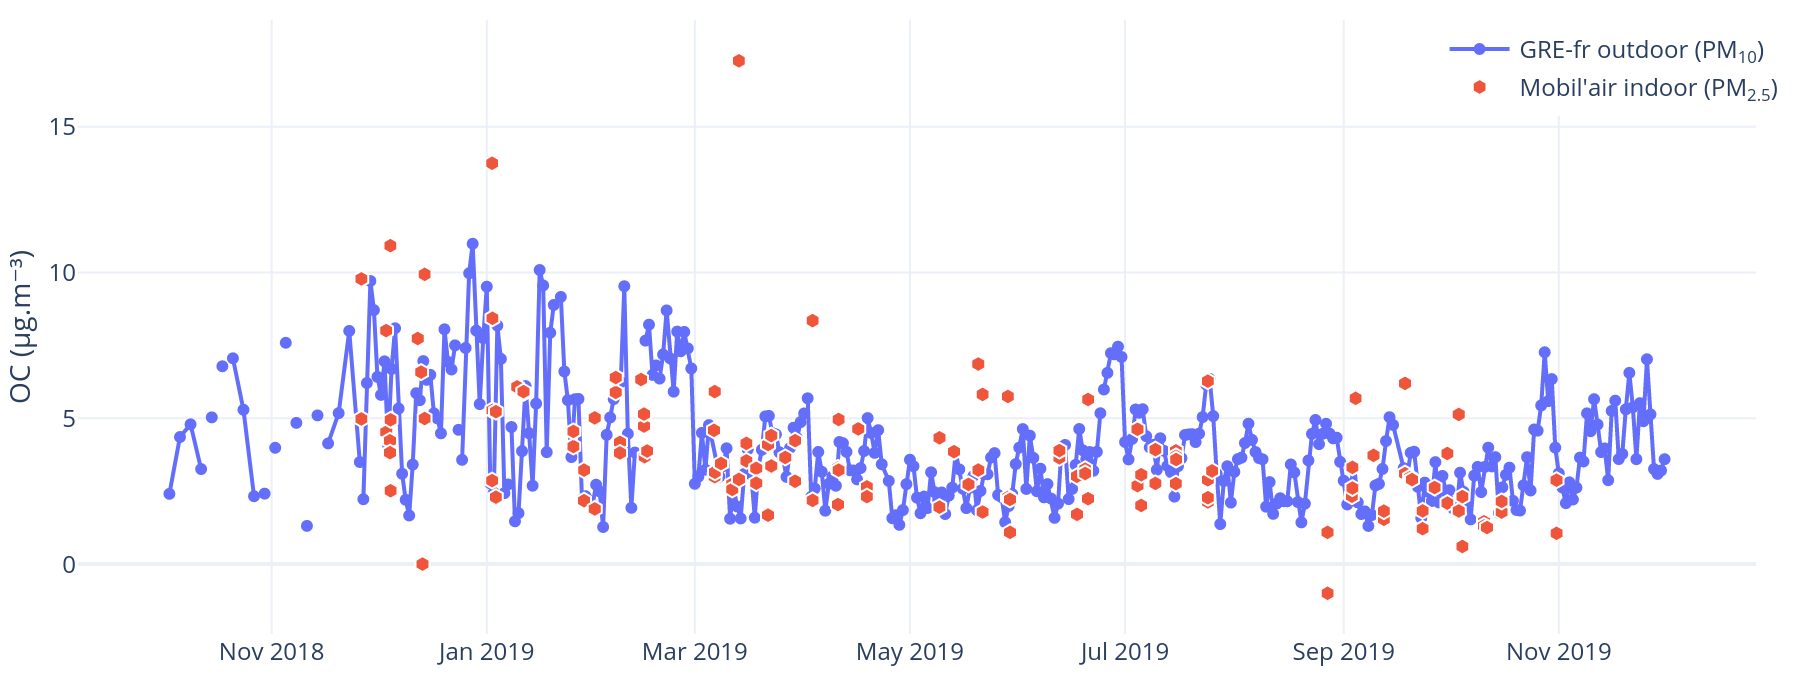
\includegraphics[width=1.\linewidth]{figures/chapter05/OC_mobilair.png}
%     \caption{Mesure de l'OC en air extérieur (station de GRE-fr) et intérieur chez les
%     participants de l'étude sur la métropole grenobloise.}%
%     \label{fig:figures/chapter05/OC_mobilair}
% \end{figure}

% Concernant les mesures personnelles, la figure~\ref{fig:figures/chapter05/personnal_OP}
% présentes la confrontation des mesures de la station GRE-fr et personnelles pour l'année
% 2015, 2016 et 2017. Bien que l'on observe toujours un cycle saisonnier pour le \POAAv{} et
% \PODTTv{} personnel, son amplitude est plus faible que celui du \POv{} d'extérieur. Aussi,
% alors que l'on a montrée dans section~\ref{sub:pm10_pm2_5} que le \POv{} des \PMdc{} est
% toujours plus faible que celui des \PMdix{} lorsqu'il proviennent de la même station de
% prélèvement, ce résultat n'est pas retrouvé pour le \POv{} personnel. Notamment, le \POv{}
% personnel en été est plus élevés que le \POv{} de l'air extérieur, indiquant des sources
% de PO différente entre air extérieur et air ``personnel''.
%
% \begin{figure}[ht]
%     \centering
%     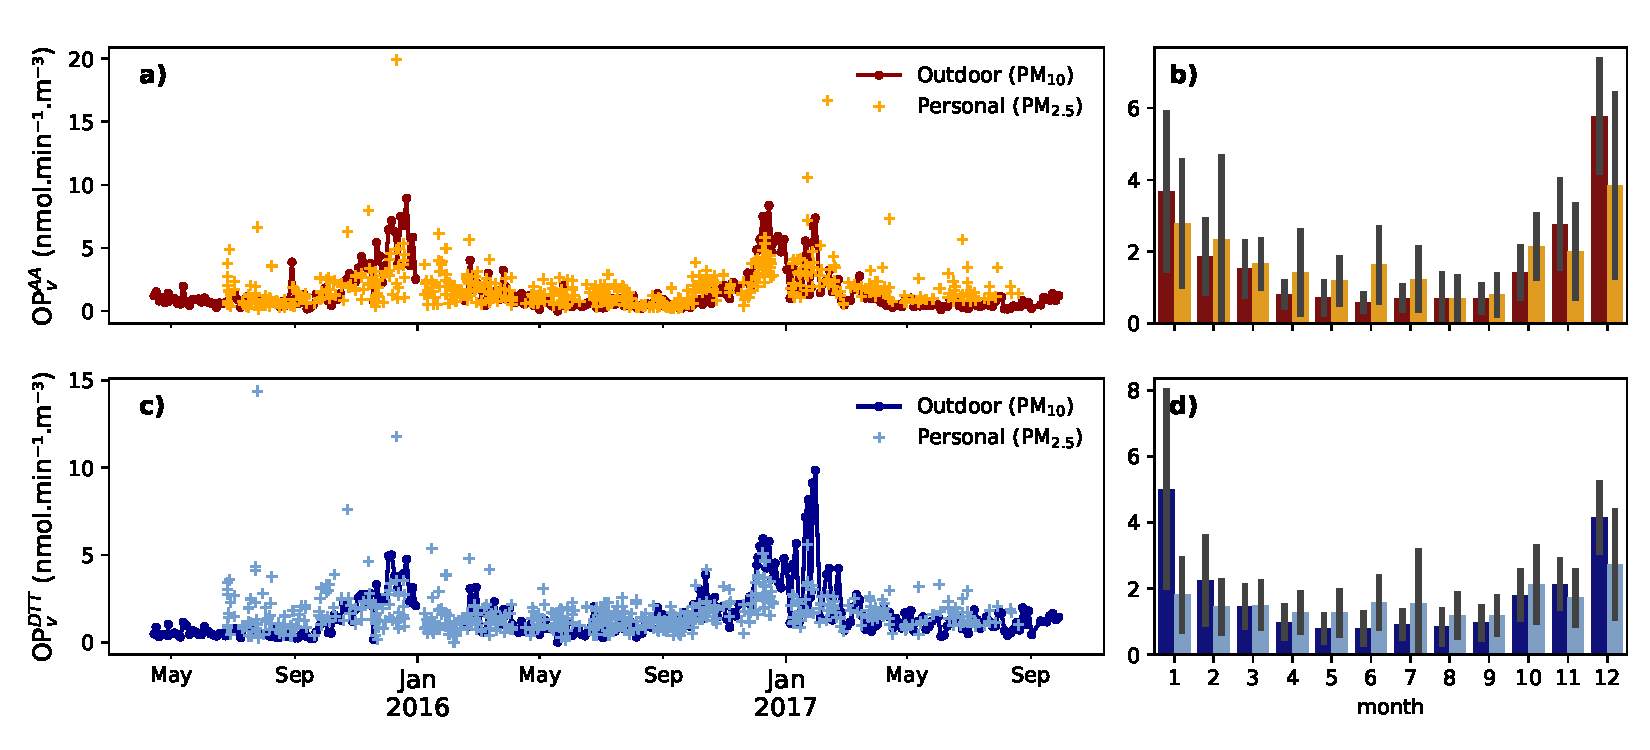
\includegraphics[width=1.0\linewidth]{figures/chapter05/personnal_OP.pdf}
%     \caption{Mesures de \POAAv{} et \PODTTv{} en extérieur (station GRE-fr) et
%     personnelles des sujets de la cohortes SEPAGES. La moyenne et l'écart type par mois
% sont présentés en b) pour le \POAAv{} et d) pour le \PODTTv. L'orange représente le
% \POAAv{} et le bleu le \PODTTv{}. Les prélèvements en extérieur sont en foncés et personel
% en clairs.}%
%     \label{fig:figures/chapter05/personnal_OP}
% \end{figure}

% \subsection{Étude épidémiologique -- cohorte SEPAGES}
%
% La cohortes SEPAGES nous permet une caractérisation précise de l'exposition personnelle
% maternelle en lien avec un ensemble conséquent de variables phénotypiques du nouveau-né.
% De façons similaire à l'étude de \cite{ouidirEstimation2015}, l'effet de l'exposition aux
% \ce{NO2}, concentration massique des \PMdc mais surtout aux \POAAv{} et \PODTTv{} est en
% cours d'étude par \cite{borlazaPersonalinprep.}.
% Grâce à cette étude, le pouvoir prédictif de la métrique de la masse ou du PO des \PMdc{}
% sur le petit poids de naissance ou la circonférence crânienne, parmi d'autres variables,
% pourra être évaluer.
%
% De même, la thèse d'Anouk Marshal débutant à l'automne 2020 aura pour objectif d'établir
% un modèle de \textit{land use regression} (LUR) sur Grenoble et périphérie afin de
% quantifier l'importance de l'environnement géographique pour la mesure du PO et
% l'exposition personnel, en lien avec les effets sanitaires observées dans la
% cohortes SEPAGES.


\bigskip

L'ensemble de ces différents travaux, déjà engagés, donnent des perspectives de recherche
intéressantes et s'inscrirtont en partie dans les travaux futurs de mon post-doctorat.
